\section{Les règles du jeu}

	\begin{frame}
	\frametitle{Les règles du jeu}
	\framesubtitle{Descriptif du jeu}
	
	\begin{block}{Le jeu}
		\begin{itemize}
			\item Jeu de société
			\item Jeu de plateau stratégique avec planification des actions
		\end{itemize}
	\end{block}
	
	\begin{block}{Résumé des règles}
		\begin{itemize}
			\item 20 villages avec des ressources et des commandes sur certains
			\item Les joueurs choisissent leur village de départ
			\item À chaque tour, planifier 6 actions afin de pouvoir récupérer des ressources et honorer des commandes
			\item Après chaque commande honorée, 2 récompenses parmi 3
			\item Les récompenses permettent d'augmenter le score économique, politique ou religieux
		\end{itemize}
	\end{block}
	
	\end{frame}


	\begin{frame}
		\frametitle{Les règles du jeu}
		\framesubtitle{Éléments du jeu sur le plateau}
		
		\begin{figure}[h]
		\centering
		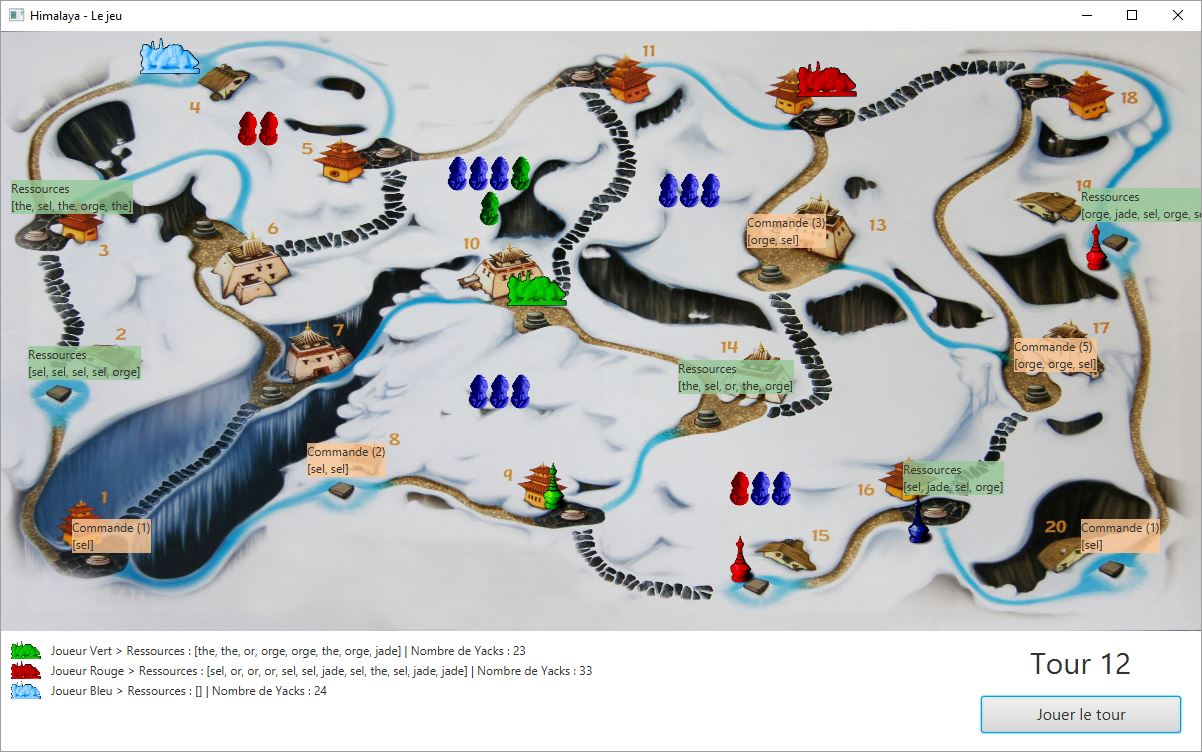
\includegraphics[width=1\linewidth]{images/etat_jeu_avance}
		\label{fig:plateau}
		\end{figure}
	
	\end{frame}

